\documentclass[9pt]{extarticle}

\usepackage[utf8]{inputenc}
\usepackage[T1]{fontenc}
\usepackage{lmodern}
\usepackage{graphicx}
\usepackage{color}
\usepackage{hyperref}
\usepackage{amsmath}
\usepackage{amsfonts}
\usepackage{epstopdf}
\usepackage[table]{xcolor}
\usepackage[a4paper, total={6in, 10in}]{geometry}
\usepackage{enumitem}
\usepackage[export]{adjustbox}


\graphicspath{ {./Figures/} }

\begin{document}

{\huge Andrew Sivaprakasam | Final Project - Progress Report 2}
\begin{center}
Final Project Repo: \url{https://github.com/sivaprakasaman/BME_511_FinalProject} \\
\end{center} 

\underline{Current State of the project:}\\ 
%
%\begin{enumerate}
%\item \underline{Evaluate Stimulus Quality: } The stimuli provided from the Philharmonia database seem to be appropriate and of good quality. There are enough instruments with A4 pitch to asses timbre. I am planning to select an A4 pitch from Banjo, Clarinet, Flute, Trombone, and Violin. Consistent with previous work, the distribution of energy within the harmonics seems to contribute strongly to timbral characteristics. As for investigating articulation and expression, there are several different sounds available, but to start simple the violin \textit{martele} and \textit{spiccato} sounds may be good. More percussive instruments (i.e. tambourine) may be a better way to assess expression since they are not centered around a particular pitch (and have very clear envelope characteristics). See attached spectrograms.
%
%\item \underline{Model Implementation/apPSTH analysis}: The BEZ2018 Model is working, and I'm able to get PSTHs for a stimulus of interest. Still playing with parameters and looking into what they do. 
%
%\item \underline{Evaluating the Question/What metrics to use: } Still working on this. The apPSTH measures and Satya's code provide a good basis for studying ENV and TFS, but I'm still trying to quantify how well ENV and TFS are coded. I'm thinking I need to look at how highly the PSD of the ENV auditory nerve responses are correlated with the PSD of the ENV of the stimulus and  a similar metric for TFS. Or, I could see how the well the PSD of AN TFS/ENV responses to music-noise chimaeras and non-chimaeras are correlated. I'm still thinking this through. Goal is to have this a good bit more fleshed out by next week. I think the question will be more focused on timbral \textit{coding} rather than \textit{perception}, since \textit{perception} would probably require behavioral data.
%\end{enumerate}

Starting to get things a little bit more thought through (but have a little bit of a ways to go). I intially thought studying timbral perception might be better aided by using music-noise chimaeras, but I don't think this is necessary to answer my current questions. Ideally, I would have conducted a perceptual study similar to Smith et al. to study whether instrumental \& articulation recognition depend primarily on TFS or ENV cues. This would have provided insight on what specifically would be best to study using the spectrally-specific apPSTH measures Satya has developed for neural spikes and ephys data.  \\

However, since the goal of this project is to learn more about spike train analysis, I will carry on with the plan of using the BEZ2018 code and apPSTH measures to look at TFS/ENV specific responses. The chimaera code isn't needed for this case, since apPSTHs give us the ability to study physiological responses to both TFS and ENV characteristics.  \\

I have been able to get the BEZ2018 code working with my stimuli (see below), and am in the process of deriving PSD measures as a function of carrier frequency/fine structure (in this case CF = A4 = 440 Hz) and modulation frequency (nonstationary and variable between instruments/articulation) coding. After getting these PSDs, I can make some observations about how the power spectra in the TFS/ENV compare with the spectrum of the original signal (using cross-correlation?) as a function of CF. Additionally, I can look at measures such as the total power in the harmonics as a function of CF. I will probably have more ideas on what analytics to use once I have derived the PSD measures and can see how the spectra appears to vary. \\

\textbf{Figures:}\\

\centering
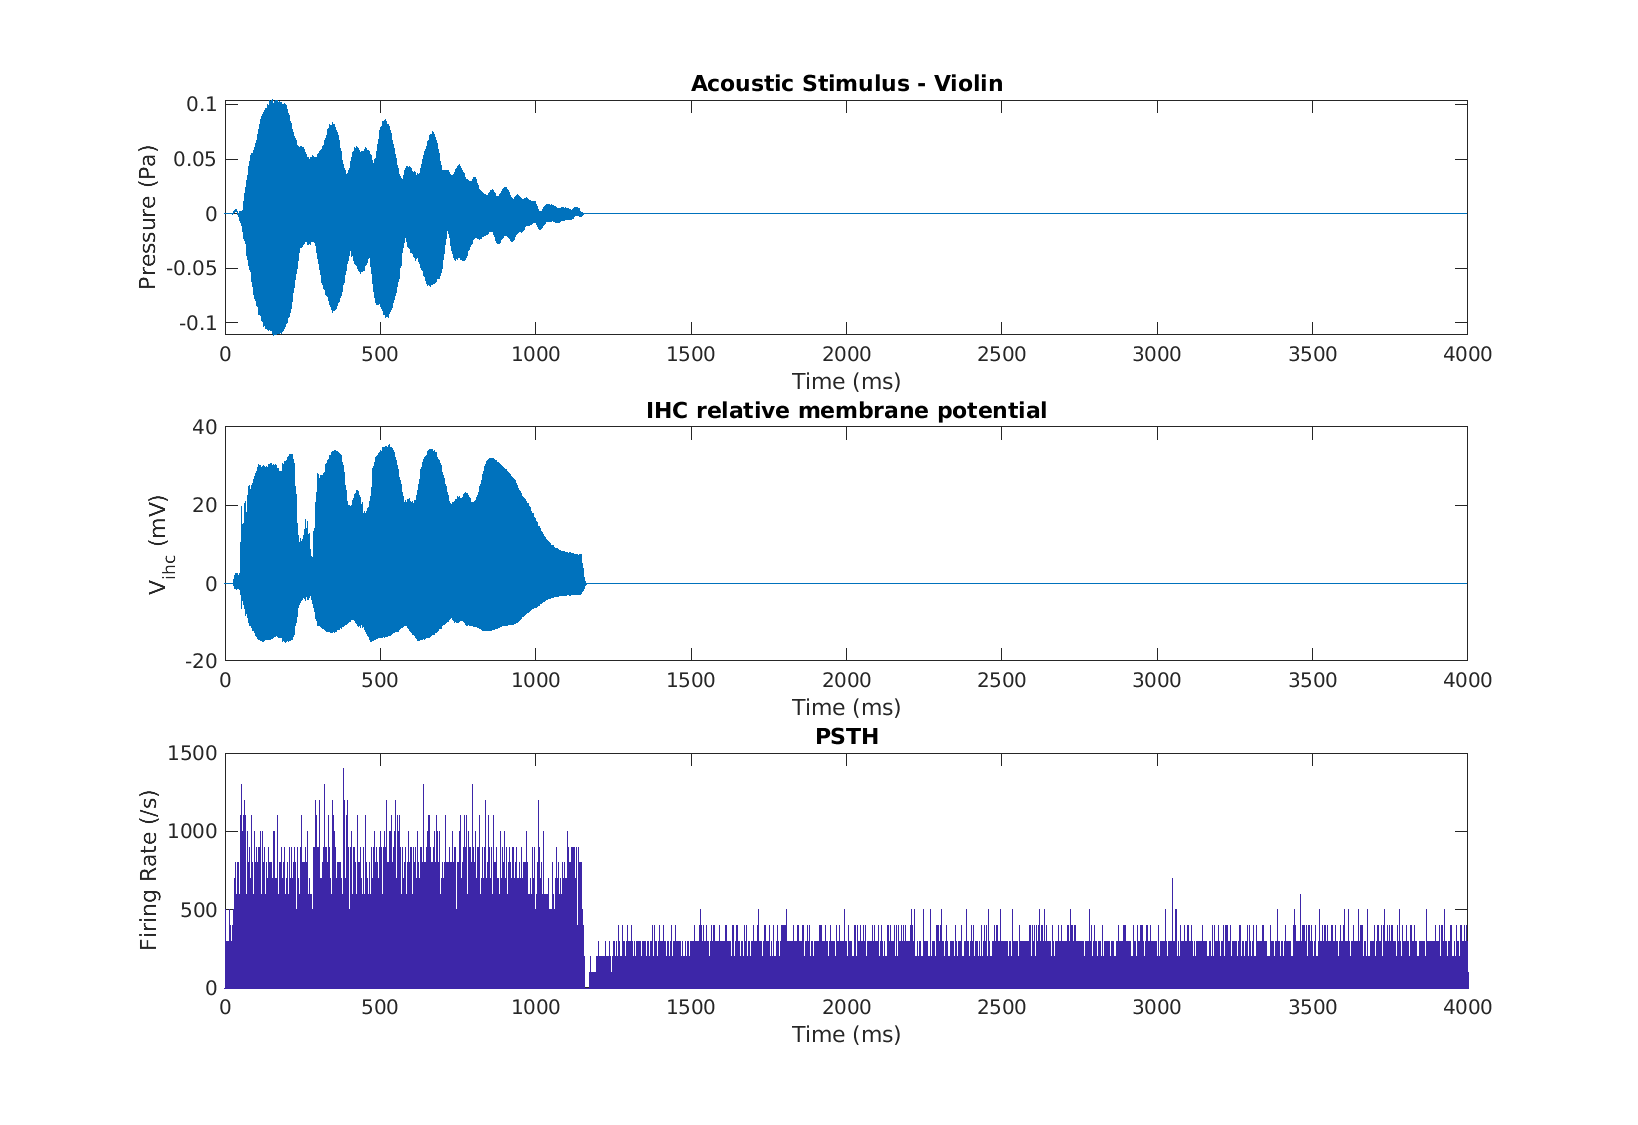
\includegraphics[width = .49\textwidth]{violin_psth}
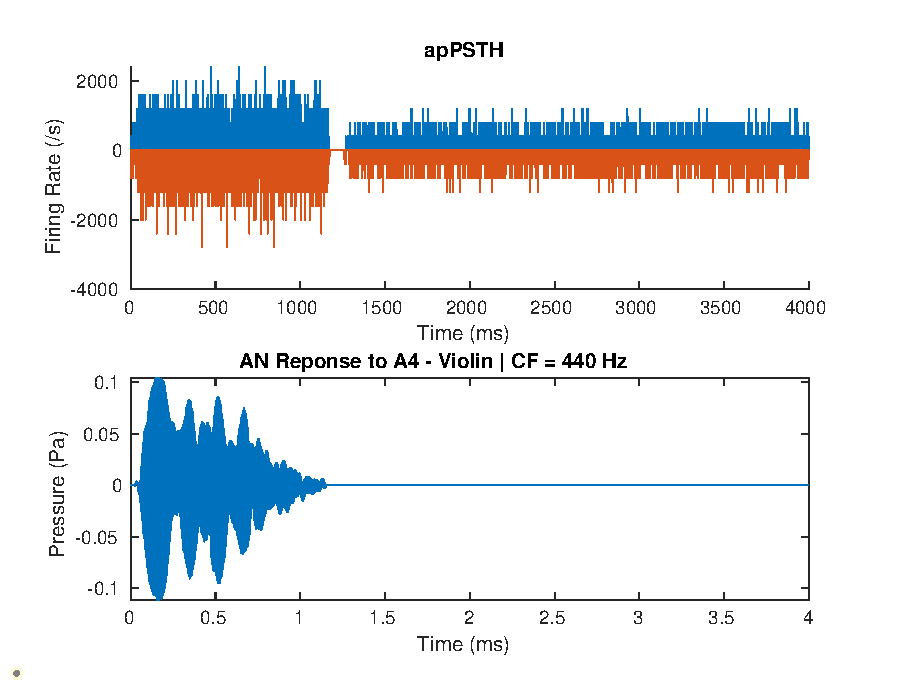
\includegraphics[width = .45\textwidth]{violin_psth_withsig_CF440}
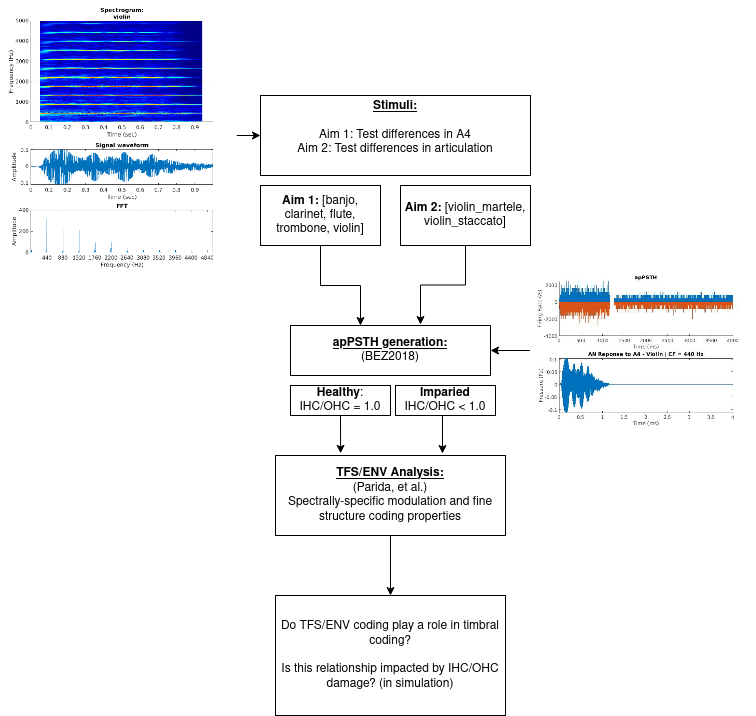
\includegraphics[width = .6\textwidth]{progress2_fig}
%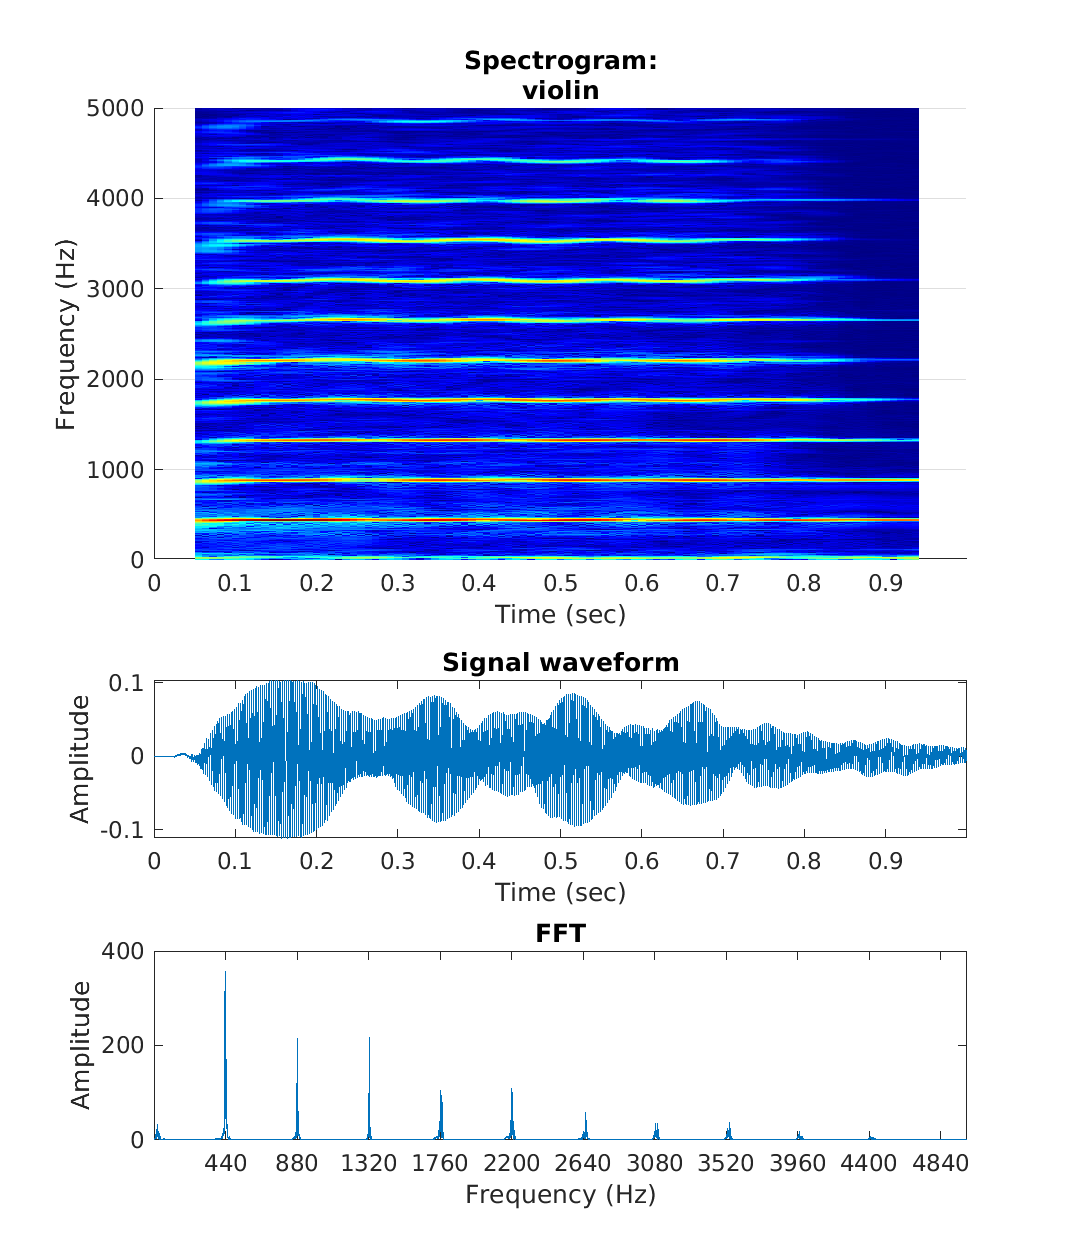
\includegraphics[width = .3\textwidth]{spectrogram_violin}\\
%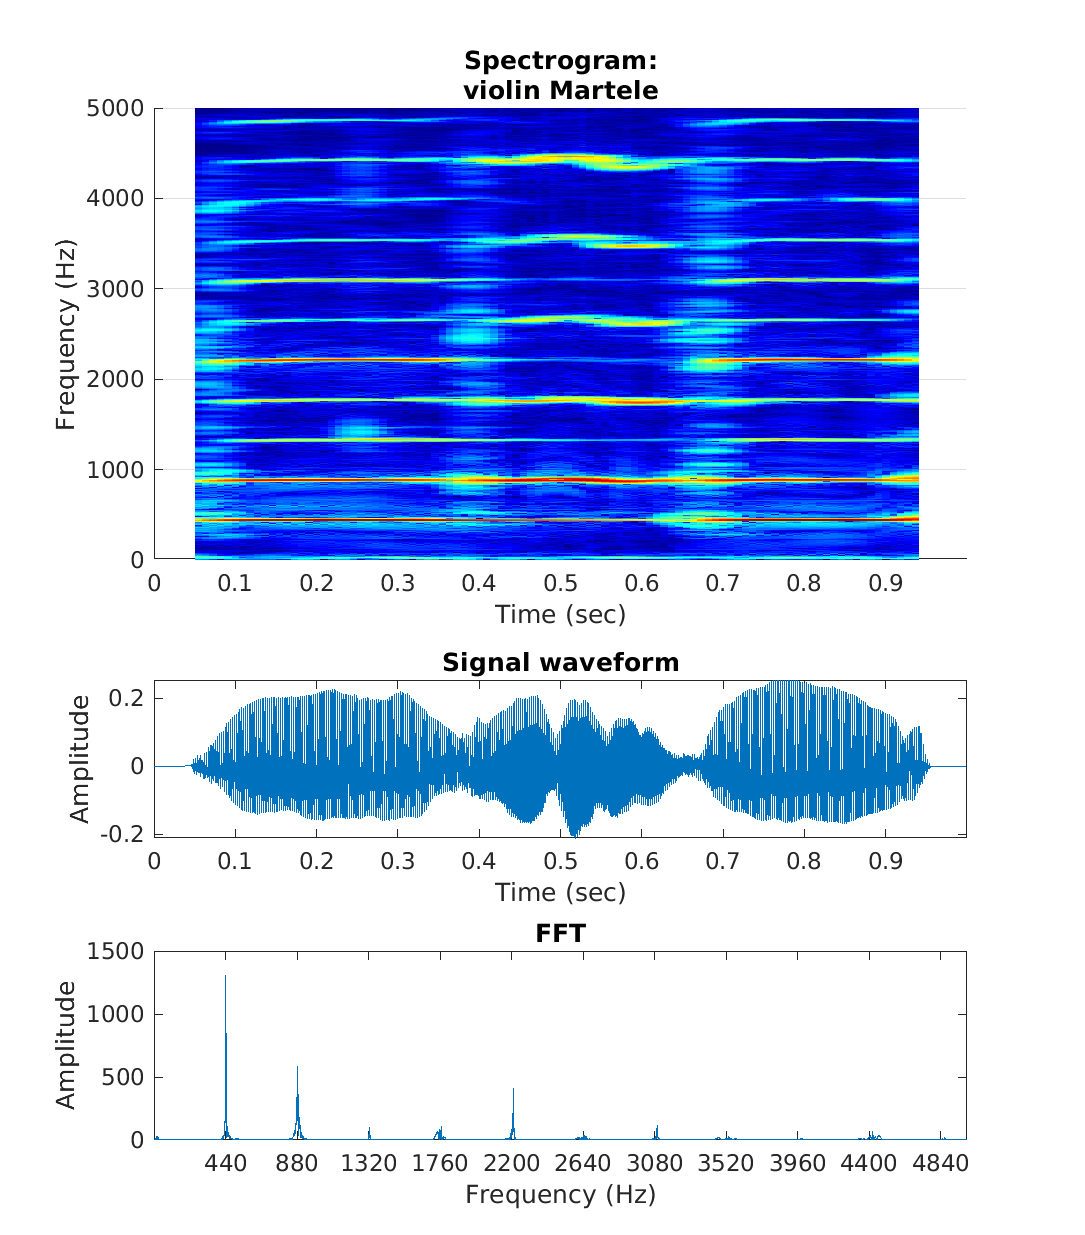
\includegraphics[width = .3\textwidth]{spectrogram_violin_phrase_forte_arco-martele}
%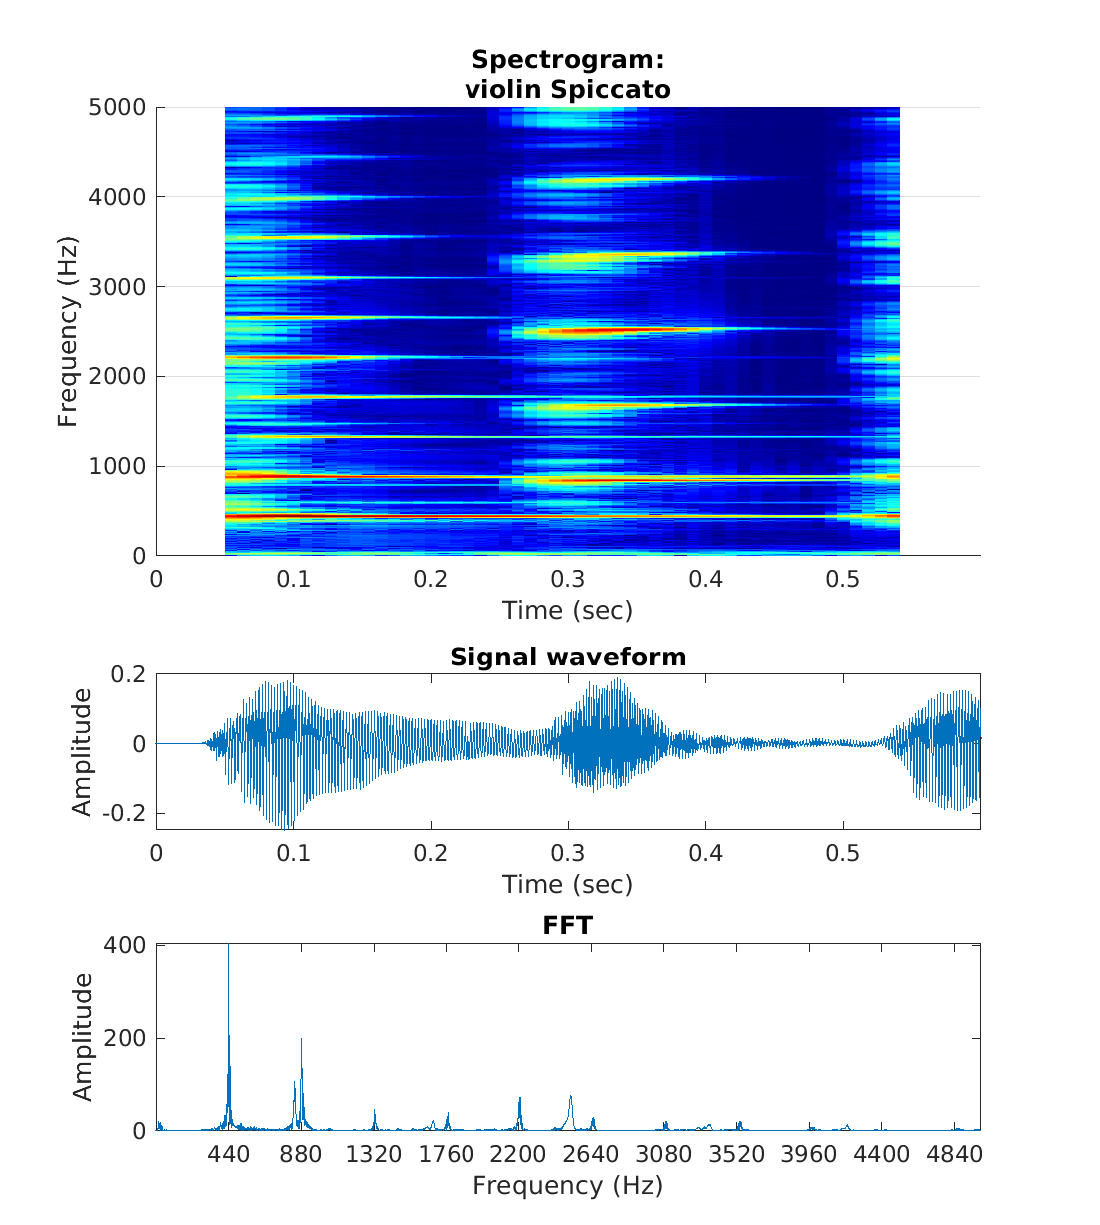
\includegraphics[width = .3\textwidth]{spectrogram_violin_phrase_forte_arco-spiccato}



\end{document}
